\documentclass[11pt,xcolor=svgnames]{beamer}
\usepackage{natbib,setspace}
\mode<presentation>

% replaces beamer foot with simple page number
\setbeamertemplate{navigation symbols}{}
%\setbeamerfont{frametitle}{series=\bfseries}
\setbeamercolor{frametitle}{fg=Black}

\setbeamertemplate{footline}{
   \raisebox{5pt}{\makebox[\paperwidth]{\hfill\makebox[20pt]{\color{gray}\scriptsize\insertframenumber}}}}

\graphicspath{{/green/Dropbox/inputs/},{/Users/mtaddy/Dropbox/inputs/}}

% colors
\newcommand{\theme}{\color{Maroon}}
\newcommand{\bk}{\color{black}}
\newcommand{\rd}{\color{DarkRed}}
\newcommand{\fg}{\color{ForestGreen}}
\newcommand{\bl}{\color{blue}}
\newcommand{\gr}{\color{black!50}}
\newcommand{\sg}{\color{DarkSlateGray}}
\newcommand{\nv}{\color{Navy}}
\setbeamercolor{itemize item}{fg=gray}

% common math markups
\newcommand{\bs}[1]{\boldsymbol{#1}}
\newcommand{\mc}[1]{\mathcal{#1}}
\newcommand{\mr}[1]{\mathrm{#1}}
\newcommand{\bm}[1]{\mathbf{#1}}
\newcommand{\indep}{\perp\!\!\!\perp}
\def\plus{\texttt{+}}
\def\minus{\texttt{-}}

% spacing and style shorthand
\setstretch{1.1}

\begin{document}

\setcounter{page}{0}
{ \usebackgroundtemplate{\includegraphics[height=\paperheight]{phoenix}}
\begin{frame}[plain]
\begin{center}

{\bf \LARGE \theme }

\vskip .25cm
{\bf \huge \theme Measuring Rhetoric \bk\vskip .2cm \Large Statistical Language Models in Social Science }

\vskip 1cm
Matt Taddy,  Chicago Booth


\vfill
{\texttt{faculty.chicagobooth.edu/matt.taddy/research}}

\end{center}
\end{frame} }

\begin{frame}
{History: \theme Text as data}

Social science text-as-data from the 1960s: \\~~~author identification in the Federalist papers.
\begin{center}
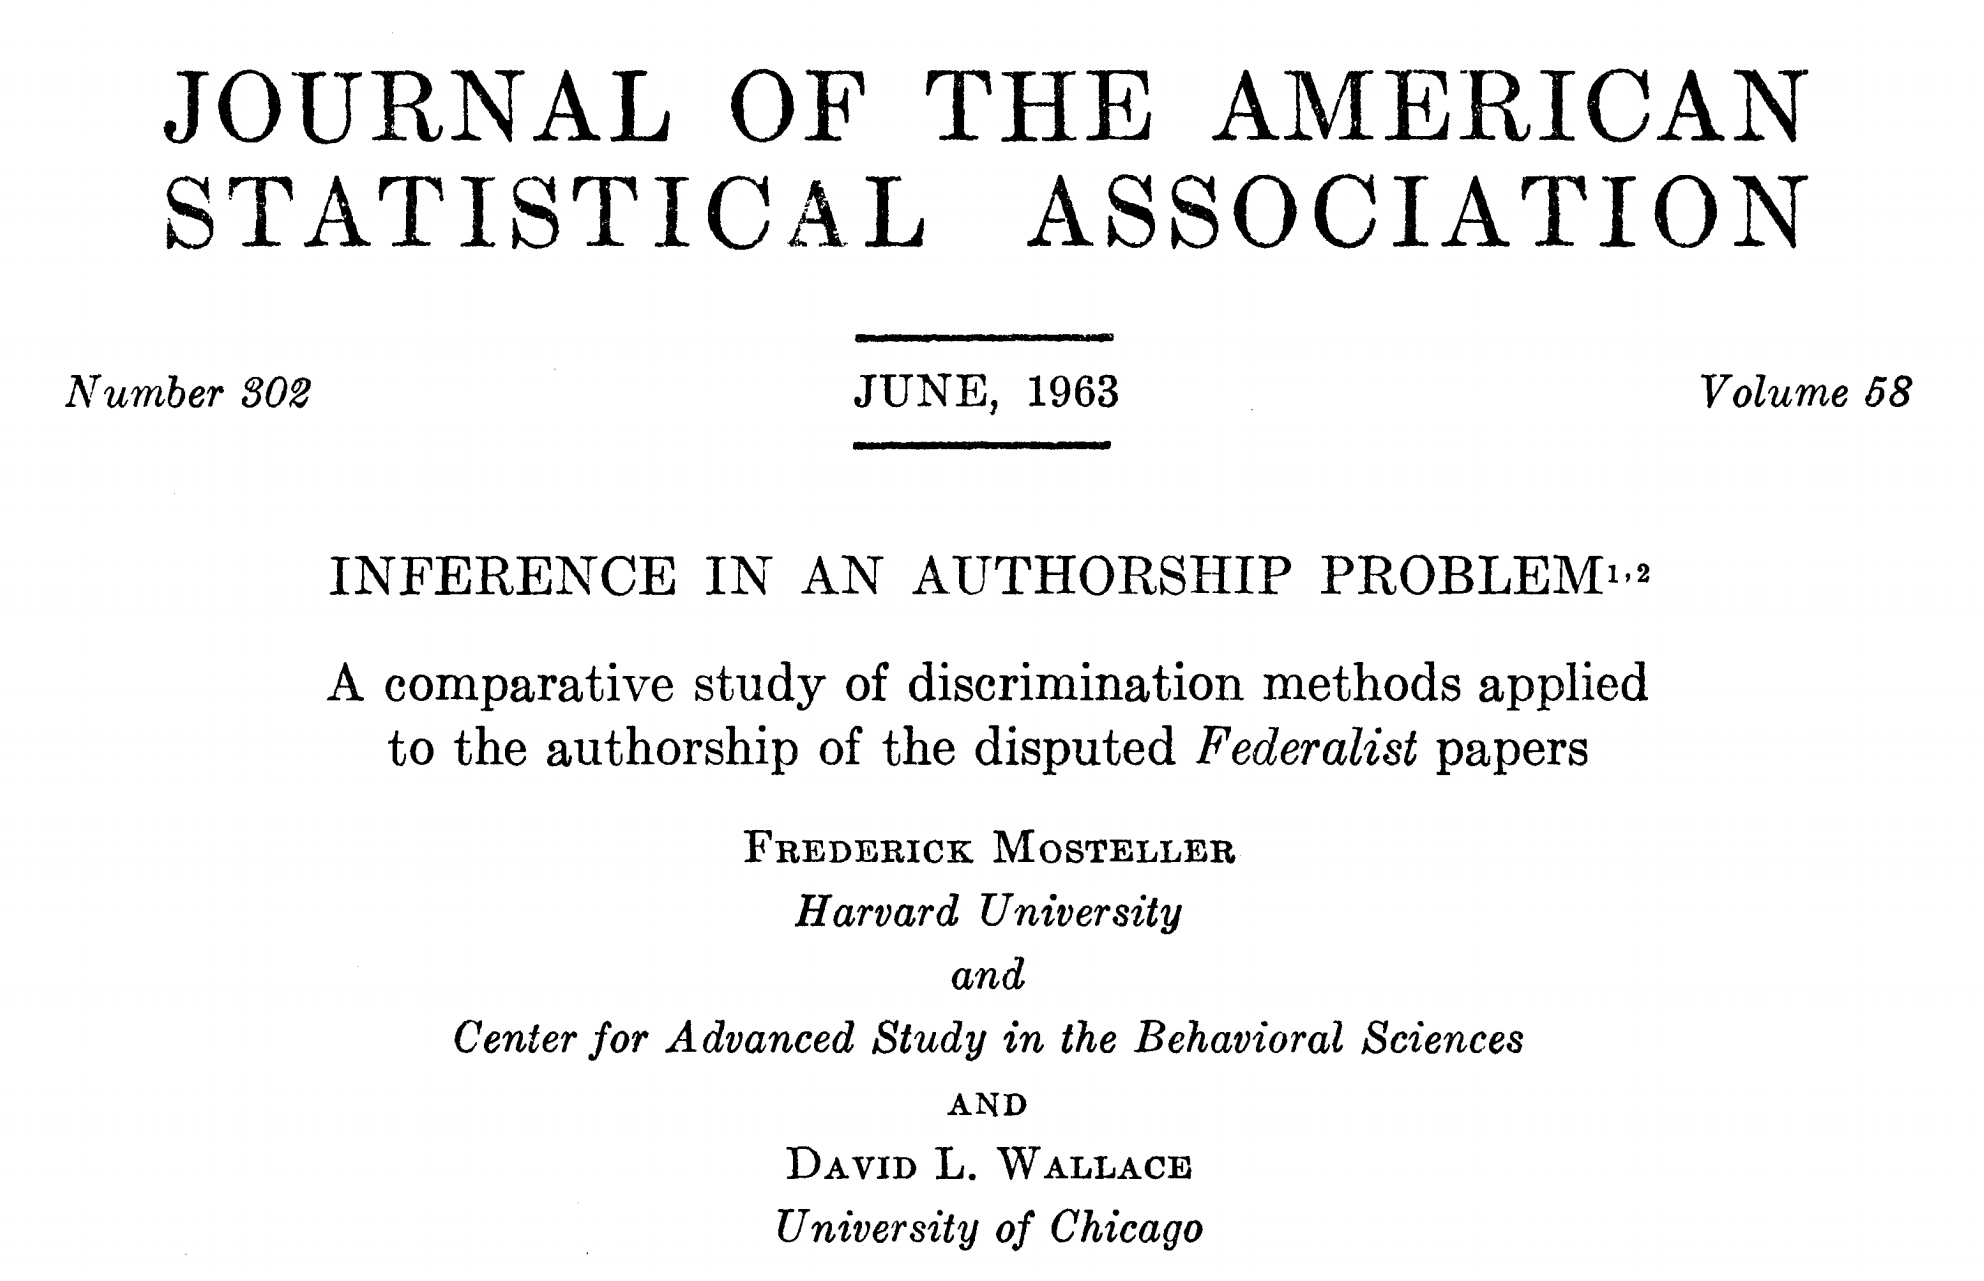
\includegraphics[width=3.75in]{../graphs/mostellerwallace}
\end{center}

\vskip -.5cm

\end{frame}

\begin{frame}


M{\tt+}W count words in papers by Hamilton and Madison,
\begin{center}
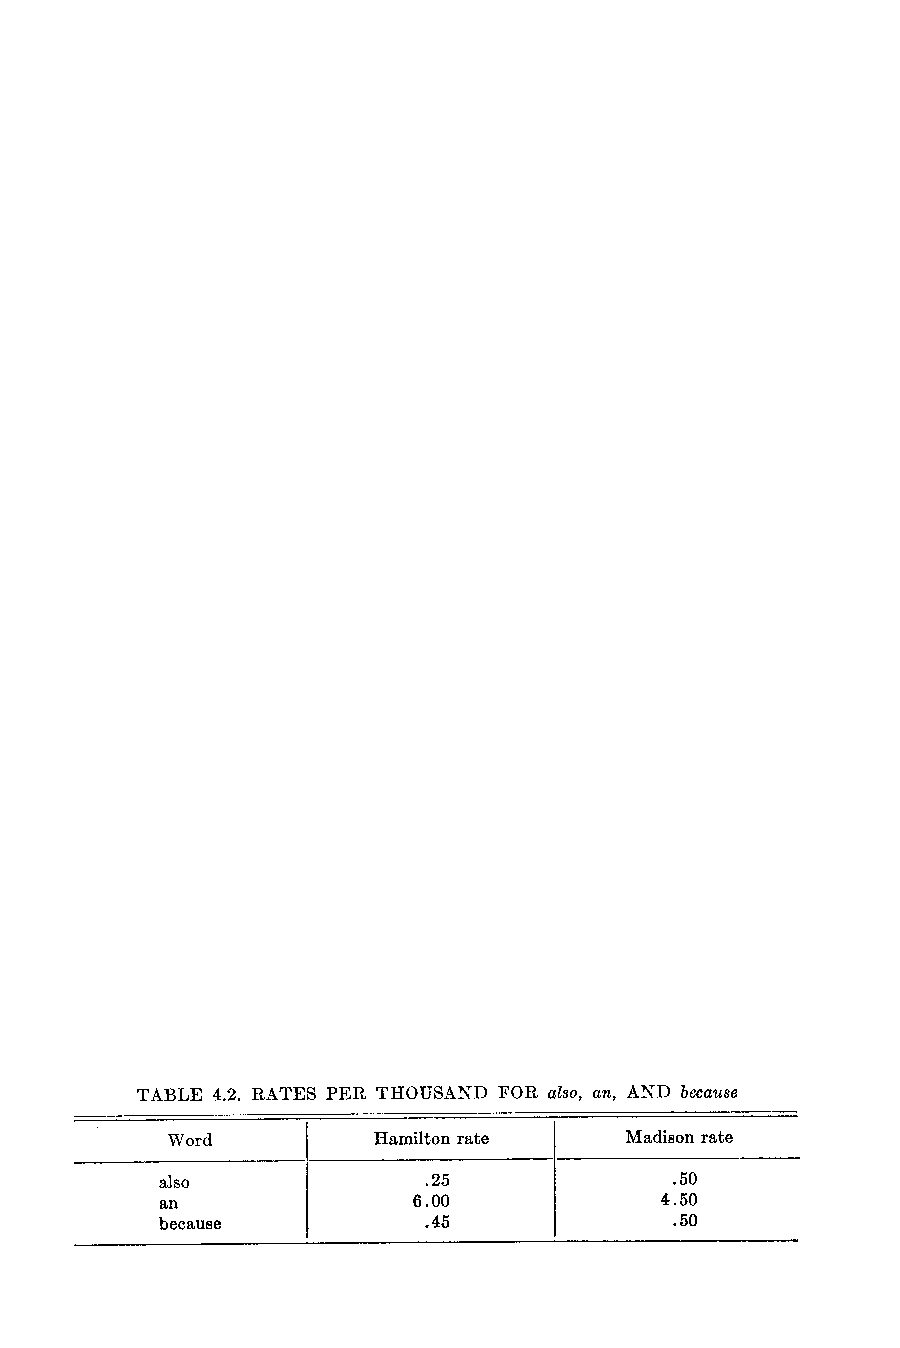
\includegraphics[width=4.25in]{../graphs/mostellertab}
\end{center}


then fit models for counts$|$author {\gr (essentially what I use today!)},
and use Bayes rule to predict authors$|$counts on disputed work.

{\large \nv\[\mr{p}(\text{Hamilton}\mid \text{text}) \approx 
\frac{\mr{p}(\text{text} \mid \text{Hamilton})}
{\mr{p}(\text{text} \mid \text{Madison}) + \mr{p}(\text{text} \mid \text{Hamilton})}
\]}

\end{frame}


\begin{frame}{
The `{\theme bag of words}'}

\vskip .25cm
 A `word' is a self-contained meaningful token...

\begin{itemize}
\item Actual words: `all', `world', `stage', `:-)', `{\tt \#textdata}'.
\item n-grams: `merely players' (bi), `men and women' (tri)
\item complicated clauses: parts of speech, act-of-god.
\item user selections on a website, domain ids in browser history 
\end{itemize}

All we do is count them.

\vskip .5cm

{\nv The remains state of the art!}

\vskip .1cm
Treat tokens for each doc as an i.i.d. sample. 

\vskip .1cm
{\theme Document $i$ is summarized by counts $c_{ij}$ for tokens $j=1...d$.}

\vskip .1cm
Dumb but works: extra rules aren't worth their complexity.

\end{frame}

\begin{frame}
{Text as data \bk in Social Science}

\vskip .25cm
There's been an explosion of interest from social scientists.

 \vskip .25cm
Until very recently, one used pre-defined dictionaries.


\vskip .25cm
{Picking words: culturomics, Michel et al, Science 2011.}
\begin{center}
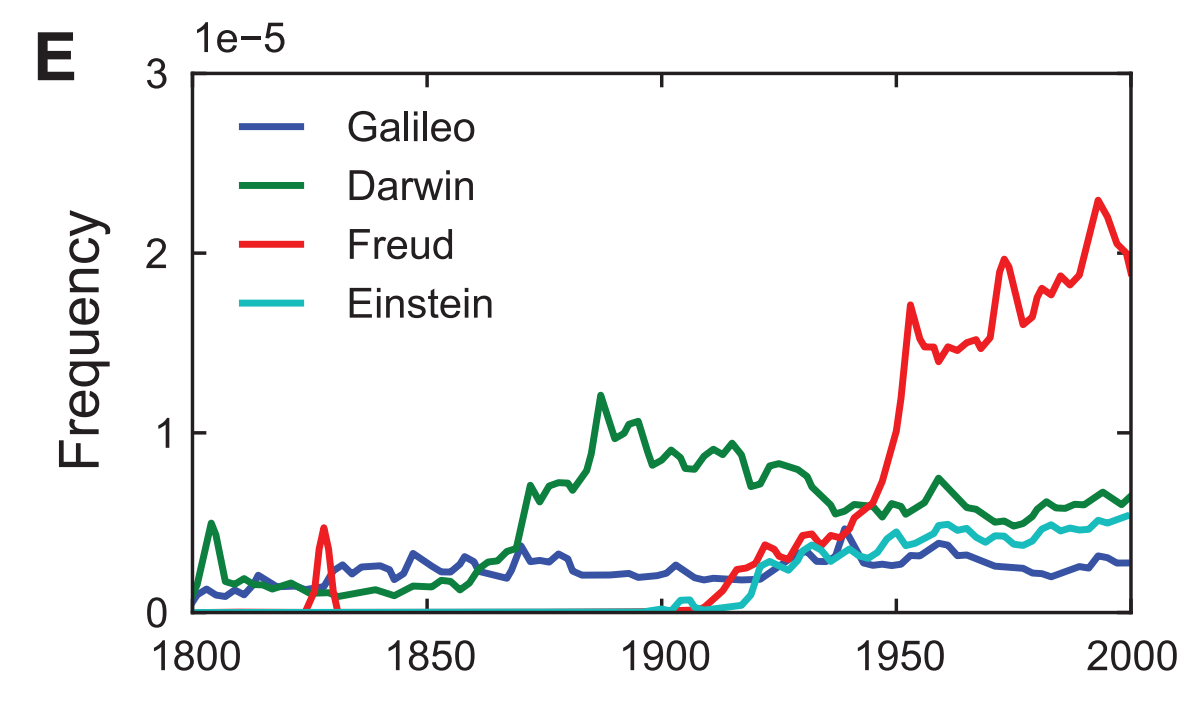
\includegraphics[width=2in]{../graphs/culturomics}
\end{center}


Psychosocial dictionaries, such as Harvard GI in {\it Tetlock 2007, Giving Content to Investor Sentiment} and others: 
\begin{center}
{\color{DarkGreen} able, abundant, accept} vs 
{\color{DarkRed} abandon, abrupt, absurd}.
\end{center}

\end{frame}

\begin{frame}
{Topic Models}

\vskip .25cm
Techniques from stats and ML are beginning to filter through and researchers are estimating relationships {\it from the data}.

\vskip .25cm  
A large area of research has developed around {\it topic models} 
\[\nv
\bm{c}_i \sim \text{MN}( \omega_{i1} \bs{\theta}_1 + \ldots + \omega_{iK} \bs{\theta}_K, m_i)
\]
{a multinomial with probabilities $\sum_k \omega_{ik}\bs{\theta}_{k}$ and size $m_i= \sum_jc_{ij}$.}

\vskip .25cm
{\gr\hfill\it (Latent Dirichlet Allocation; Blei, Ng, Jordan 2003)~~~}

\vskip .5cm
This is a factor model for count data.


\end{frame}

\begin{frame}

Topics provide low-D structure, which the SS interprets.

{\gr Especially common in PoliSci; King, Grimmer, Quinn, ...}


\begin{center}
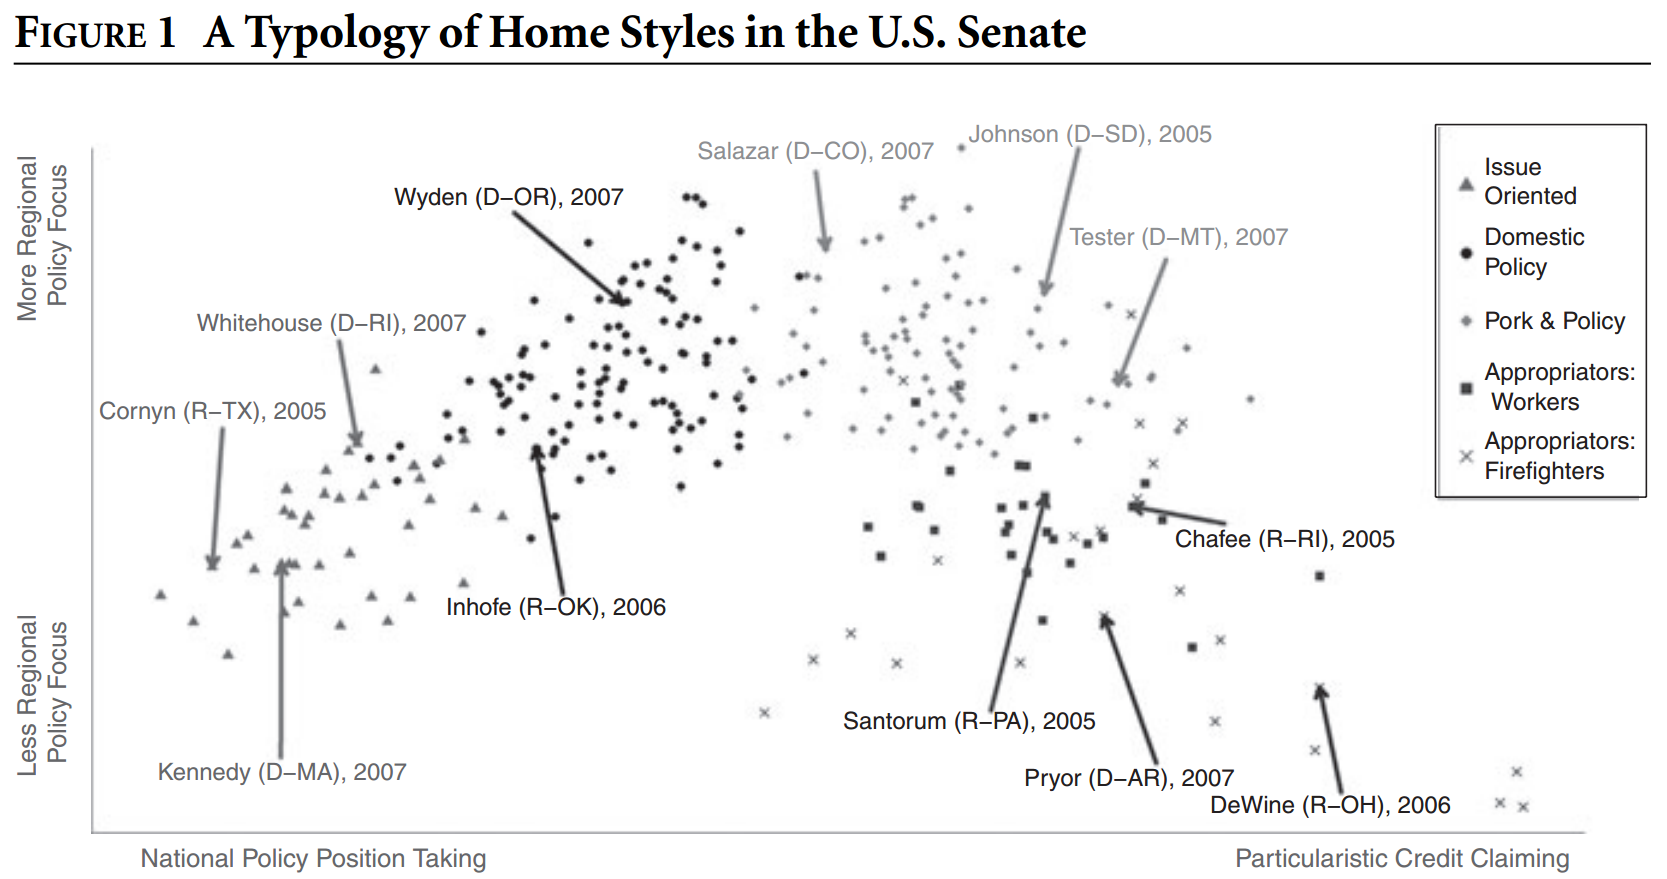
\includegraphics[width=3.75in]{../graphs/grimmer}
\end{center}


{\it Grimmer 2013:}  fit latent topics in press releases \\(e.g., `Iraq', `Infastructure') then investigate who uses what topic.

\end{frame}

\begin{frame}
{Structured topic models}

The basic topic model finds {\it dominant sources of variation} in $\bm{C}$.

\vskip .1cm
In SocSci, this is often not what we're seeking (needle \texttt{+} haystack).

\vskip .5cm
There is a huge industry on extensions to topic models that push the topics to be relevant or interpretable for specific questions. \\\hfill{\gr supervised TM, dynamic TM, structural TM, IR TM ...~~~~~}

\vskip .5cm
These model weights ($\omega$) and topics ($\theta$) as functions of covariates.

\vskip .1cm
Lots of good and interesting work.



\end{frame}

\begin{frame}
{Multinomial Regression}

Instead of jumping straight to latent structure, perhaps we can answer our questions by regressing the text onto observables `$\bm{v}$'.


\vskip .5cm
Massive response {\nv logistic regressions}: 


\vskip .2cm ~~~~$\bm{c}_i \sim \mr{MN}(\bm{q}_i, m_i)~~\text{with}~~
q_{ij} = e^{\eta_{ij}}/\sum_l e^{\eta_{il}}$

\vskip .2cm ~~~~${\nv  \eta_{ij} = \alpha_j + \bm{v}_i'\bs{\varphi}_{j}}$ is a `log intensity'  {\gr $\approx \mathrm{E}\log(c_{ij}/m_i)$}

\vskip .5cm
This is a regression like any other.   

\vskip .2cm
We will be estimating {\it partial correlations}, can build {\it random effects} and {\it interactions} into $\bm{v}$, ...  all our familiar regression ideas apply.

\vskip .25cm
{\gr \it MN Inverse Regression \texttt{+} rejoinder, 2013.  Political Sentiment on Twitter, 2013.  Distributed MN Regression, 2015.}
\end{frame}

\begin{frame}
{Distributed Multinomial Regression}

{\gr A regression like any other, except the response is super HD. }

We approximate the MN likelihood with {\it independent} Poissons: 
{\large \nv \[
c_{ij} \sim \mr{Po}(~m_ie^{\eta_{ij}}~)
\]}
$\Rightarrow$ you can estimate each regression fully independently!

\vskip .5cm
This works because MN dependence is {\it only  induced by  totals}.

% \vskip -.35cm
% \[
% \mr{MN}\left(\bm{c}_i;~\bs{\pi}_{i}/\Pi_i,
% ~m_i\right) = \frac{\prod_j
% \mr{Po}\left(c_{ij};~\pi_{ij}\right)}
% {\mr{Po}\left(m_i;~\Pi_i\right)}~~\text{where}~~\Pi_i = \sum_j \pi_{ij}
% \]

\vskip .25cm
DMR is equivalent to MN logit in a variety of simple examples,\\ and is shown empirically to perform well in more complex settings.

\vskip .25cm
Everything in distribution: estimation, penalization, selection ...
\end{frame}

\begin{frame}

More precisely, start from the Poisson:
\[
c_{ij}\stackrel{ind}{\sim}\mathrm{Pois}\left(\exp\left[\mu_{i}+\eta_{ij}\right]\right)
\]
where $\mu_{i}$ is a `verbosity' nuisance parameter.


\vskip .1cm
This model leads to 
\[
\Pr\left(\mathbf{c}_{i}\mid m_{i}\right)=\frac{\prod_{j}\mathrm{Po}\left(c_{ij};\exp\left[\mu_{i}+\eta_{ij}\right]\right)}{\mathrm{Po}\left(m_{i};\sum_{l}\exp\left[\mu_{i}+\eta_{il}\right]\right)}=\mathrm{MN}(\mathbf{c}_{i};\mathbf{\,\, q}{}_{i},m_{i})
\]
Thus, given $m_i$, Poisson and MN imply the same  model.

\vskip .1cm
DMR fixes $\hat \mu_i = \log m_i$, so LHD factorizes to independent Poissons.


\vskip .5cm{\gr
More generally: for Big Data, consider using plug-in [marginal] estimates of parameters about which you have little uncertainty.  \\Focus computation on the bits that are hard to measure.}


\end{frame}

\begin{frame}
{Yelp Reviews}

We'll illustrate using {\theme publicly available} review data from Yelp.

\vskip .2cm
\begin{itemize}
\item $n=$ 215,879 reviews on 11,535 businesses by 43,873
users.
\item taken around Phoenix AZ on January 19, 2013.
\item $d=$ 13,938 words in more than 20 reviews.  
\end{itemize}

\vskip .2cm
The reviews are marked with review, business, and user attributes: number of stars, user and business star averages, business type (333 overlapping), and {\theme the number of funny/useful/cool votes.}

\end{frame}

\begin{frame}

Each {\it word-j} intensity regression equation has
\[
\eta_{ij} = \alpha_j + \bm{a}_i'\bs{\varphi}_j^a+ \bm{b}_i'\bs{\varphi}_j^b
\]
where we've resolved the meta-data attributes $\bm{V} = [~\bm{A} ~\bm{B}~]$\\ into variables of primary interest  and those viewed as controls
\begin{itemize}
\item[\bk \bf a:] star and vote counts; 11 dimensional.
\item[\bk \bf b:] 400 categories and 11,500 business random effects.
\end{itemize}


\vskip .5cm
Estimate parameters to minimize the penalized Poisson deviance
\[
\hat\alpha_j,\bs{\hat\varphi}_j = 
 \mathrm{argmin} \left\{l(\alpha_j,\bs{\varphi}_j) + n \lambda \left[\sum_k \omega^a_{jk} |\varphi^a_{jk} | + \frac{1}{\tau}\sum_k \omega^b_{jk} |\varphi^b_{jk} |\right]\right\}
\]
{\gr \it one-step estimator paths for concave regularization, 2015.}
\end{frame}

\begin{frame}

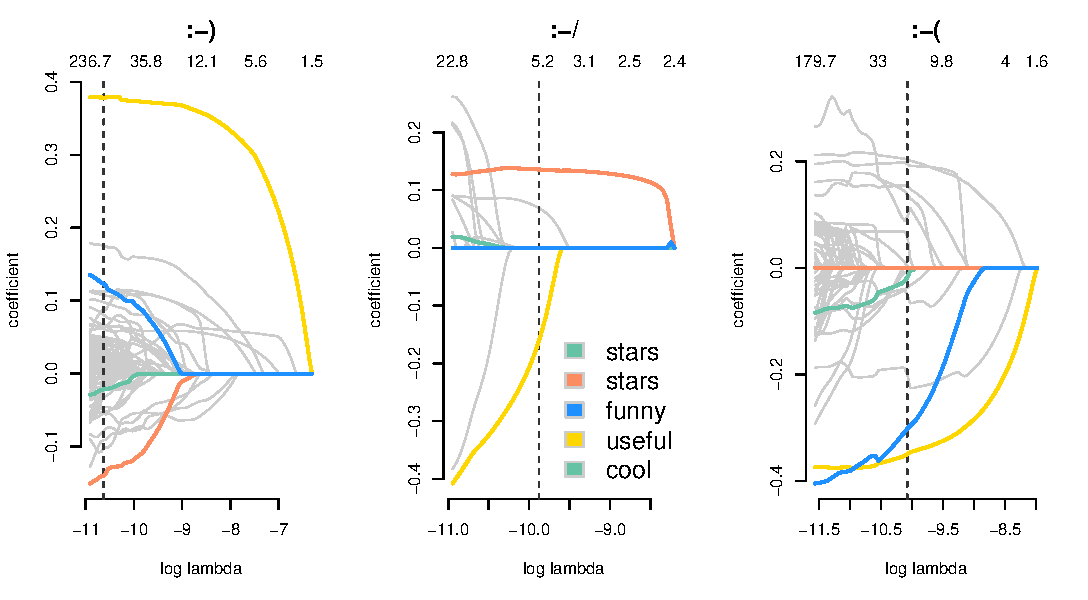
\includegraphics[width=\textwidth]{../graphs/yelp_ir_paths}

\vskip .5cm
Poisson regression regularization paths under relative weight $\tau=2$.  

AICc selection is marked.

\end{frame}

\begin{frame}

{\bf\theme Resolving correlated effects}

\vskip .2cm
Bigger $\tau$ gives fewer but {\it cleaner} nonzero terms.

{\tiny\setstretch{1.25}\color{black!80}
\hspace{-.25cm}\begin{tabular}{cll|r}
& \scriptsize $\bs{\tau}$ & \scriptsize $|\bs{\hat\varphi}|_0$ 
& \scriptsize {\bf top ten words by loading}\\
\noalign{\smallskip}
\hline
 & \multicolumn{2}{l|}{marg}    & \tiny\it great love amaz favorite deliciou best awesome alway perfect excellent \\
\scriptsize +stars & 2 & 8440 & \tiny\it  unmatch salute :-)) prik laurie pheonix trove banoffee exquisite sublime \\
 & 20 & 3077 & \tiny\it  heaven perfection gem divine amaz die superb phenomenal fantastic deliciousnes \\
 & 200 & 508 & \tiny\it  gem heaven awesome wonderful amaz fantastic favorite love notch fabulou \\
\hline
&  \multicolumn{2}{l|}{marg}   & \tiny\it  not worst ask horrib minut rude said told would didn \\
\scriptsize -stars & 2 & 8440 & \tiny\it  rude livid disrespect disgrace inexcusab grosse incompet audacity unmelt acknowl \\
 & 20 & 3077 & \tiny\it  rude incompet unaccept unprofession inedib worst apolog disrespect insult acknowl \\
 & 200 & 508 & \tiny\it  worst horrib awful rude inedib terrib worse tasteles disgust waste \\
\hline
 & \multicolumn{2}{l|}{marg}   & \tiny\it  you that know like your yelp ... what don who \\
\scriptsize funny & 2 & 6508 & \tiny\it  dimsum rue reggae acne meathead roid bong crotch peni fart \\
 & 20 & 1785 & \tiny\it  bitch shit god dude boob idiot fuck hell drunk laugh \\
 & 200 & 120 & \tiny\it  bitch dear god hell face shit hipst dude man kidd \\
 \hline
 &  \multicolumn{2}{l|}{marginal}   & \tiny\it  that yelp you thi know biz-photo like all http :// \\
\scriptsize useful & 2 & 5230 & \tiny\it  fiancee rife dimsum maitre jpg poultry harissa bureau redirect breakdown \\
 & 20 & 884 & \tiny\it  biz-photo meow harissa www bookmark :-/ http :// (?), tip \\
 & 200 & 33 & \tiny\it  www http :// com factor already final immediate ask hope \\
\hline\end{tabular}}

\vskip .5cm
I think $\tau=20$ strikes a good balance here.

\vskip -.5cm
\end{frame}

\begin{frame}

{\bf \theme Sufficient Reduction}

\vskip .5cm
What is the funny/useful/cool content of a review?

\vskip .5cm
Coefficients $\bs{\Phi}$ are a linear map from text to attribute space.

\vskip .1cm
They provide a {\it sufficient reduction}. For example,
\[
\bm{a}_i \indep \bm{c}_i \mid
\bs{\Phi}^a \bm{c}_i, \bm{b}_i, m_i
\]
where $\bs{\Phi}^a$ are loadings relevant to our `primary interest' covariates.

\vskip .5cm
In words: the 11 dimensional $\theme \bm{z}_i = \bs{\Phi}^a \bm{c}_i$ contains all the information in the text that is {\it directly} relevant to $\bm{a}_i$, controlling for $\bm{b}_i$ and $m_i$.

\end{frame}

\begin{frame}

\footnotesize

{\bf Funniest and most useful 50-100 word review, as voted by Yelp users\\ {\gr (votes normalized by square root of review age).}}

\vskip .5cm{\it\color{black!70}\nv
I use to come down to Coolidge quite a bit and one of the cool things I use to do was come over here and visit the ruins.  A great piece of Arizona history!  Do you remember the Five C's?  Well, this is cotton country. The Park Rangers will tell you they don't really know how old the ruins are, but most guess at around 600 years plus.  But thanks to a forward thinking US Government, the ruins are now protected by a 70 foot high shelter.  Trust me, it comes in handy in July and August, the two months I seem to visit here most.  LOL.  I would also recommend a visit to the bookstore.  It stocks a variety of First Nation history, as well as info on the area.
  http://www.nps.gov/cagr/index.htm.  While you are in Coolidge, I would recommend the Gallopin' Goose for drinks or bar food, and Tag's for dinner.  Both are great!}

\end{frame}


\begin{frame}

\footnotesize

{\bf 50-100 word review with the most funny content, \\as measured by SR projection 
$\bs{z_{\texttt{funny}}} = \bs{\hat\phi}_{\texttt{funny}}'\bm{c}$.}

\vskip .25cm
{\it \nv Dear La Piazza al Forno: We need to talk. I don't quite know how to say this so I'm just going to come out with it. I've been seeing someone else. How long? About a year now. Am I in love? Yes. Was it you? It was. The day you decided to remove hoagies from your lunch menu, about a year ago, I'm sorry, but it really was you...and not me.  Hey... wait... put down that pizza peel... try to stay calm... please? [Olive oil container whizzing past head] Please! Stop throwing shit at me... everyone breaks up on social media these days... or haven't you heard?  Wow, what a Bitch!}

\vskip .75cm
{\bf most funny by $\bs{z_{\texttt{funny}}}/m$:} ~~~\textit{\nv Holy Mother of God}

\end{frame}

\begin{frame}

\footnotesize

{\bf 50-100 word review with the most useful content, \\as measured by SR projection 
$\bs{z_{\texttt{useful}}} = \bs{\hat\phi}_{\texttt{useful}}'\bm{c}$.}

\vskip .25cm
{\it \nv We found Sprouts shortly after moving to town.  There's a nice selection of Groceries \& Vitamins.  It's like a cheaper, smaller version of Whole Foods.
[biz-photo] [biz-photo] We shop here at least once a week.  I like their selection of Peppers....I like my spicy food! [biz-photo][biz-photo][biz-photo] Their freshly made Pizza isn't too bad either. [biz-photo] Overall, it's a nice shopping experience for all of us. Return Factor - 100\%}

\vskip .75cm
{\bf most useful by $\bs{z_{\texttt{useful}}}/m$:} ~~~\textit{\nv Ask for Nick!}

\end{frame}

\begin{frame}

The SR projections are based on {\it partial correlations}.  

\vskip .25cm
E.g., compare the correlation matrices
\begin{center}\vskip -.5cm
~~~~~~\begin{tabular}{r|ccccr|cccc}
 \multicolumn{4}{l}{\it attributes ($\bm{v}$)} & & 
 \multicolumn{4}{l}{\it \hskip .3cm text projections ($\bm{z}$)} \\ 
 %\multicolumn{10}{c}{}\\
\multicolumn{1}{c}{}& f & u &c & $\star$ &  \multicolumn{1}{c}{}&f & u &c & $\star$\\
\cline{2-5}\cline{7-10}
funny &  1 &  0.7 &  0.8 &   0 & \hskip .3cm funny &  1 &  -0.1 &  -0.7 &  -0.4\\
useful &  0.7 &  1 &  0.9 &   0 & \hskip .3cm useful &  -0.1 &  1 &  0.1 &  -0.2\\
cool &  0.8 &  0.9 &  1 &   0 & \hskip .3cm cool &  -0.7 &  0.1 &  1 &  0.5\\
stars &   0 &   0 &   0 &  1 & \hskip .3cm stars &  -0.4 &  -0.2 &  0.5 &  1\\
\end{tabular}
\end{center}

\vskip .5cm
SR projections make great inputs to prediction algorithms: {\theme MNIR}.

\end{frame}

\begin{frame}

{\bf Confounder Adjustment}

\vskip .1cm
Text is also a useful, but high-dimensional, control.

\vskip .25cm
For example: does a user's experience effect their review ranking?

{\gr Do they get more positive, say because of a yelp community effect?}

\vskip .25cm
{\theme Given the same review, do experienced users give more/less stars then a newbie?}
We can answer by {\it controlling} for review content.

\vskip .5cm
Treatment effect of experience on rating
\begin{itemize}
\item response attribute, $v_{iy}$, is  {\it star rating}. 
\item treatment, $v_{id}$, is the log {\it number of reviews} by the author.
\item controls are $\bm{v}_{i,-yd}$ (everything else) and $\bm{c}_i$.
\end{itemize}

\end{frame}

\begin{frame}


Given our MN language model,
\[
v_{iy},v_{id} \indep \bm{c}_i \mid z_{iy},z_{id},m_i,\bm{v}_{i,-yd}
\]
So  the {\it joint distribution} of treatment and response is independent of 
review content ($\bm{c}$) given the SR projections on each ($z_{iy},z_{id}$).

\vskip .5cm
We can control for this content, {\it and its interaction with business classification},
and estimate treatment effect $\gamma$ in 
\[
\mathrm{E}[v_{iy}] = \gamma v_{id} + f( z_{iy},z_{id},m_i,\bm{v}_{i,-yd} )
\]
This gives {\theme $\hat \gamma = 0.02$}, vs a marginal effect near zero and an effect of 0.015 conditioning on $\bm{v}_{i,-yd}$ alone.  {\gr Interacting $\bm{c}_i$ with biz class gives 5 million coefficients $\Rightarrow$ not enough degrees of freedom.}

\end{frame}

\begin{frame}
{Measuring segregation in high dimensions}

With Gentzkow\texttt{+}Shapiro, the congressional record since 1873 and a question:
{\theme ``How has  partisanship of rhetoric changed over time?''}

\vskip .5cm
The concept here is of speakers across parties:
\begin{itemize}
\item using different words to describe the same thing\\
{\tt\theme tax.cut}/{\tt\nv tax.break}, 
{\tt\theme war.on.terror}/{\tt\nv war.in.iraq}
\item choosing to focus on different substantive topics\\
{\tt\theme stem.cell}, {\tt\nv african.american}, %{\tt\nv sea.level}, 
{\tt\theme soldier.sailor}.
\end{itemize}
And doing this because of party membership or ideology.

\end{frame}

\begin{frame}

In HD, indices of segregation  can have strange properties: variation in the index is dominated by your ability to measure it.

\vskip .5cm
G\texttt{+}S 2013, {\it Slant index} on 10k most common phrases

\vskip .1cm
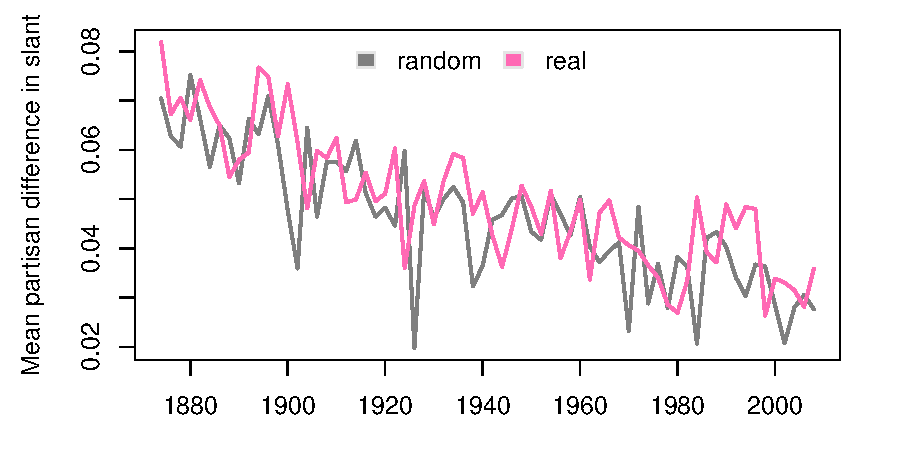
\includegraphics[width=\textwidth]{../graphs/slant_10k}

\vskip .1cm
Real is Dem v. GOP.  Random is a random permutation.
\end{frame}


\begin{frame}

In HD, indices of segregation  can have strange properties: variation in the index is dominated by your ability to measure it.

\vskip .5cm
G\texttt{+}S 2011, {\it Isolation index} on 10k most common phrases

\vskip .1cm
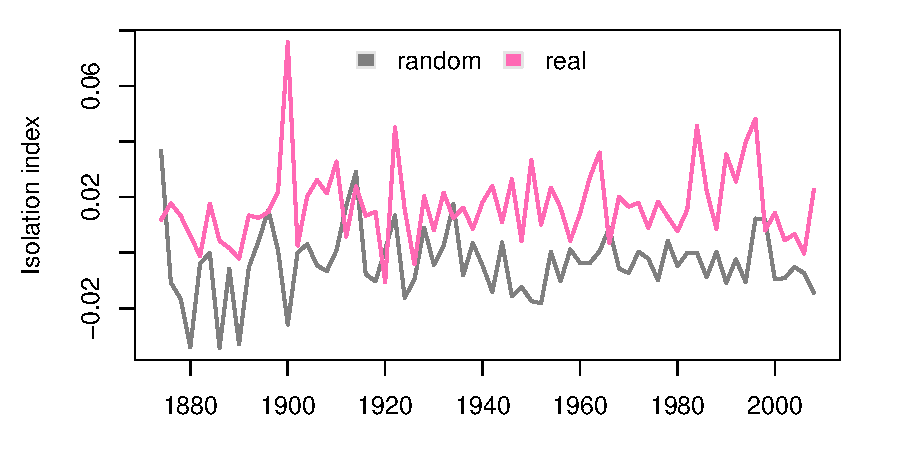
\includegraphics[width=\textwidth]{../graphs/isolation_10k}

\vskip .1cm
Real is Dem v. GOP.  Random is a random permutation.
\end{frame}


\begin{frame}

Instead, we write down a {\theme multinomial choice model} with intensities
\[
\eta_{ijt}  =\alpha_{jt}+\mathbf{u}_{it}'\boldsymbol{\gamma}_{j}+\varphi_{jt}'r_{it} 
\]
So that $\eta_{ijt}$ is the mean utility of phrase 
$j$ for speaker  $i$ in session $t$.

\vskip .25cm
$\mathbf{u}_{it}$ are measured attributes of speaker $i$ in session  $t$ (e.g., state, chamber), excluding the Republican party membership indicator $r_{it}$.


\vskip .5cm
The SR projection for (Republican) partisanship is $z_{it} = \bs{\varphi}_{t}'\bm{c}_{it}$.

\vskip .25cm
Here, this is the expected utility gain to a Republican relative to a Democrat from speaking exactly like speaker $i$
  in session $t$.

\end{frame}

\begin{frame}

We use a spline model to allow $\bs{\varphi}_{t}$ to change slowly in time.

\vskip .5cm
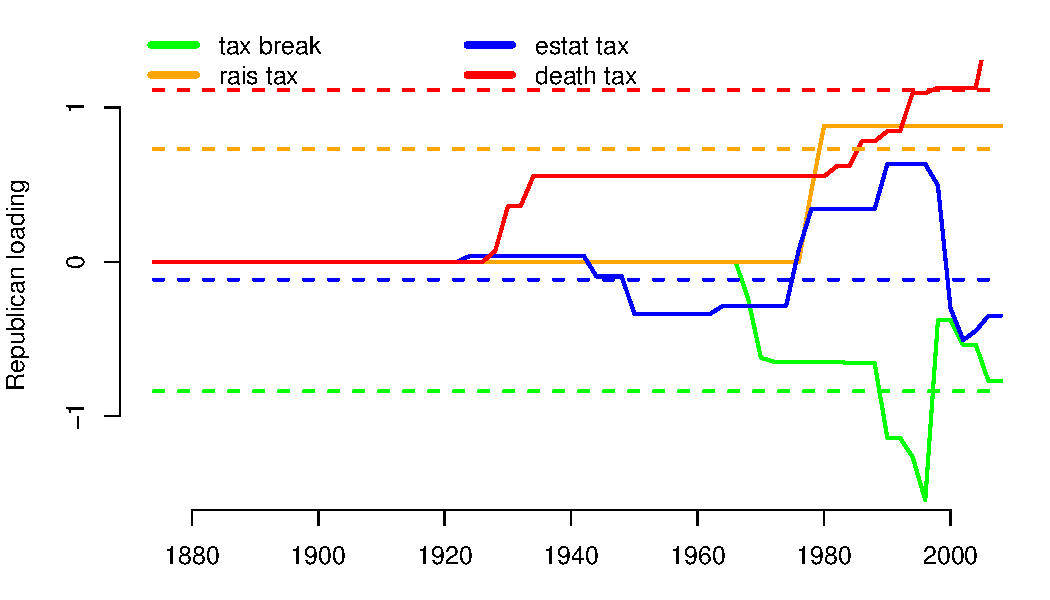
\includegraphics[width=\textwidth]{../graphs/loaded_tax}

\end{frame}


\begin{frame}

We use a spline model to allow $\bs{\varphi}_{t}$ to change slowly in time.

\vskip .5cm
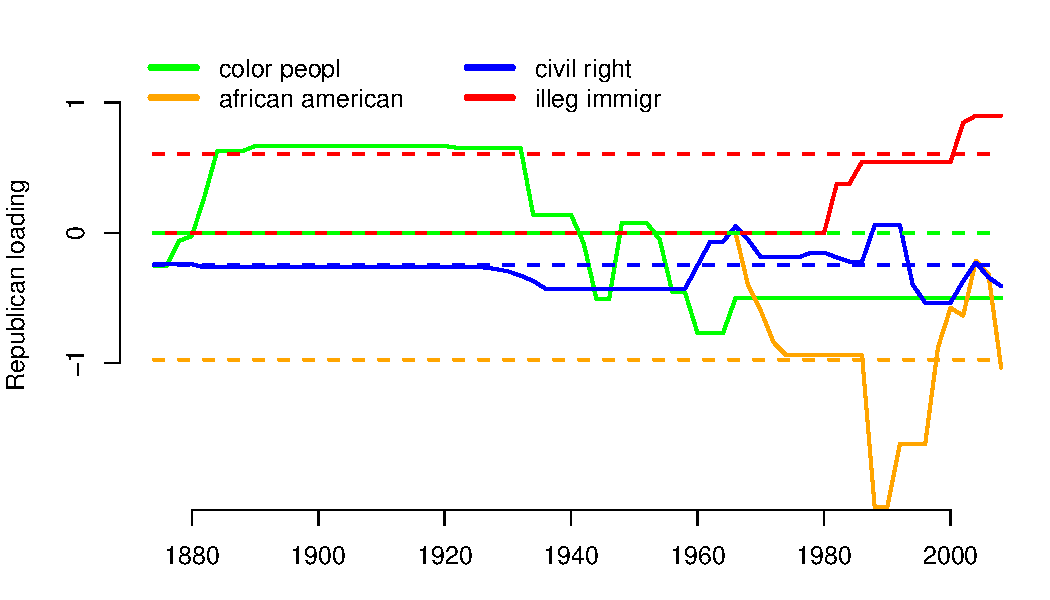
\includegraphics[width=\textwidth]{../graphs/loaded_race}

\end{frame}

\begin{frame}

SR measures {\it preferences} in a structural model.  

\vskip .1cm
Segregation of preferences is $\bar z_{\texttt{gop},t} - \bar z_{\texttt{dem},t}$.


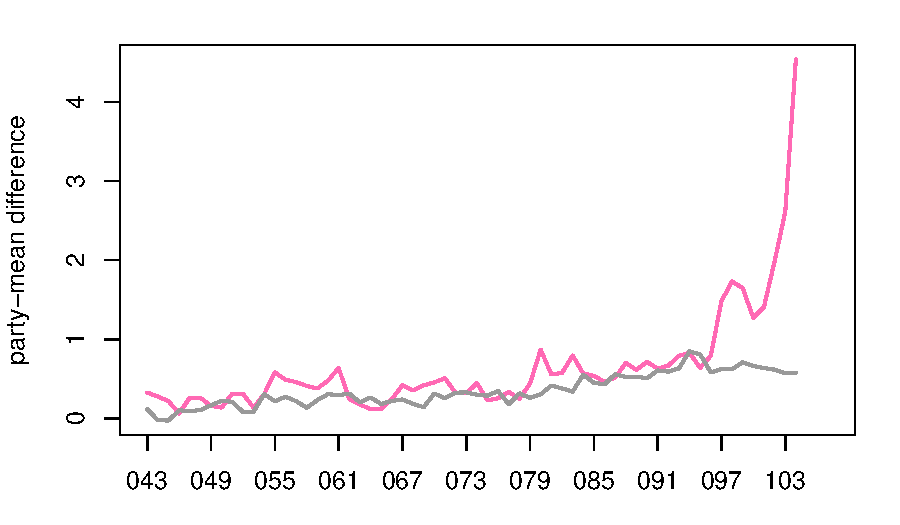
\includegraphics[width=\textwidth]{../graphs/bic-polars}

We see a clear pattern: partisanship explodes after Carter.

\end{frame}

\begin{frame}
{Messaging and Negotiation on eBay.com}

eBay has a `{\theme best offer}' button; a buyer can use this to circumvent the auction or fixed price sale, and make a direct offer to the seller.

\vskip .5cm
We track the communication.  

\vskip .5cm
After controlling for parameters of the transaction {\gr (item, buyer offer, seller/buyer info, ...)} {\theme what language leads to a higher probability of a seller responding with a deal or counteroffer?}

\vskip .5cm
We can use the results to educate buyers, give templates/examples, or generate hypotheses on bargaining behavior.

\end{frame}

\begin{frame}

To isolate the targeted effect, we first remove what was predictable from the 0/1 response, $y:$ `did seller respond to buyer?'

\vskip .5cm
Fit $p_i = \mr{p}(y_i=1 | \bm{x}_i)$ as an {\it Empirical Bayesian Forest} ($\approx$ an RF).

{\gr $\bm{x}$: buyer, seller, item attributes (even includes sale title topics). }

\vskip .5cm
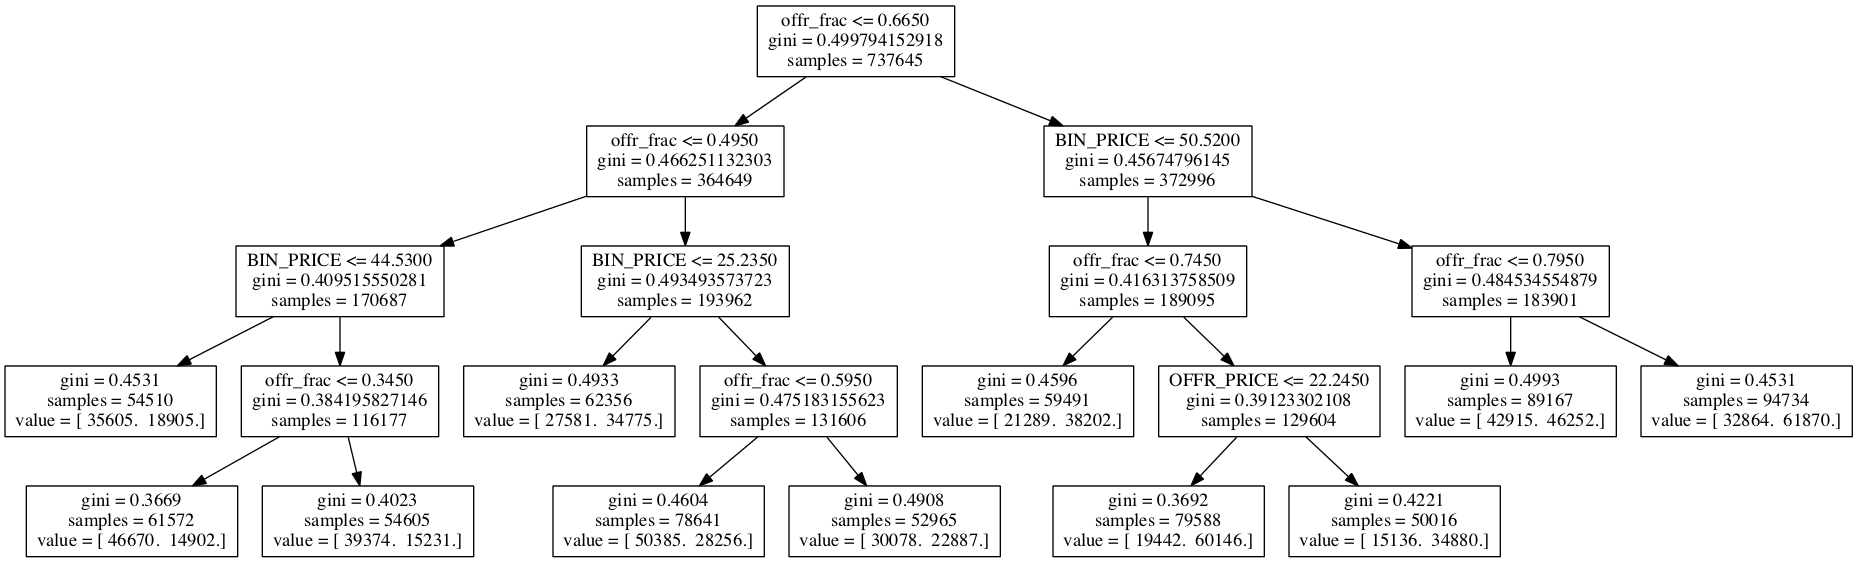
\includegraphics[width=\textwidth]{../graphs/botrunk}

\vskip .5cm
Then we look at the SR projection from text onto $r_i = y_i - \hat p_i$.

\end{frame}

\begin{frame}

First, without the synthetic treatment residual: 

\vskip .1cm
Log intensity $\eta_{ij} = \alpha_j + \varphi_j^y {\color{red} y_i} + \bm{x}_i'\bs{\beta_j}$, SR $z_i^y = \bm{c}_i'\bs{\varphi}^y$.

\vskip .2cm
The highest $z_i$ all showed evidence of previous deals and bundling.

The lowest $z_i$ are agressive offers, driving a hard bargain:

\vskip .5cm
{\footnotesize \nv \it \setstretch{1}
know this low but its based on what individual [product] selling

\vskip .2cm
give you two cash you ship it free its very common low end [product] has broken pin good pin youd be lucky get this real its worth melt price dont believe me its really not worth listing fees that you paid

\vskip .2cm
hi my offer basically what price guide lists individual [product] it may seem too low you but it never hurts place offer regards [name]

\vskip .2cm
do you know that clubhouse sigs fakes worthless ridiculous fake sigs thats why other ball sold they were real sigs real sigs lot better its like gehrigs wife signing his name not worth anything

\vskip -.5cm
}

\end{frame}


\begin{frame}

Now, with residual $r_i$ as treatment: 

\vskip .1cm
Log intensity $\eta_{ij} = \alpha_j + \varphi_j {\color{blue} r_i} + \bm{x}_i'\bs{\beta_j}$, SR $z_i = \bm{c}_i'\bs{\varphi}$.

\vskip .2cm
The highest $z_i$ are still previous deals and bundling.

But the lowest $z_i$ are now pleading:

\vskip .5cm
{\footnotesize \nv \it \setstretch{1}
kcollect [product] know that my offer not close what you asking cant afford pay much more than my offer but really want this pin please let me know you can make counteroffer this offer not acceptabl

\vskip .2cm
you dont like offer feel free tell me what lowest youll go on these [product] like you ive been collect since was im now hope we can reach deal wich fair both us by way they some awsome [product] !!

\vskip .2cm
hello my friend hope my offer good enough really want  [product] ... cgc going be there they grading comics also do you know how much they charge grade comic thkas greg

\vskip .2cm
last one sold on dec 26th ,, can match that price im also interested [product] was wondering how much pair ?? can have money ur account tonight we can reach deal thanks your time ,,

\vskip -.5cm
}

\end{frame}

\begin{frame}
{wrap up}

\vskip .5cm
{Big picture: \theme  Give regression a chance!}  

\vskip .1cm
Everything here -- random effects, synthetic controls, lasso variable selection, utility interpretations -- is common in regression.  

We can apply the same ideas to text via DMR.

\vskip .5cm
{\theme Future pitch:} I've been learning about the recently popular `deep' distributed language models (e.g., word2vec) that have a word's probability dependent upon its neighbors.  

\vskip .1cm
It is pretty straightforward to add covariates into these `models', and it should lead to even cleaner SR projections.  

\begin{center}
\huge
Thanks!
\end{center}

\end{frame}

\end{document}
